\chapter{Laser Joining}
\section{Laser welding (Schweißen)}


Figure \ref{fig:energy} shows the process of \textbf{deep penetration} laser welding, also known as \textbf{keyhole} welding. 
Deep penetration welding enables higher speeds.  A shielding gas is introduced to shield the join from oxygen. Addition of the gas
depends on the material, welding without gas can be faster and more flexible. 



\begin{figure}[h!]
    \centering
    \begin{subfigure}[b]{0.45\textwidth}
        \centering
        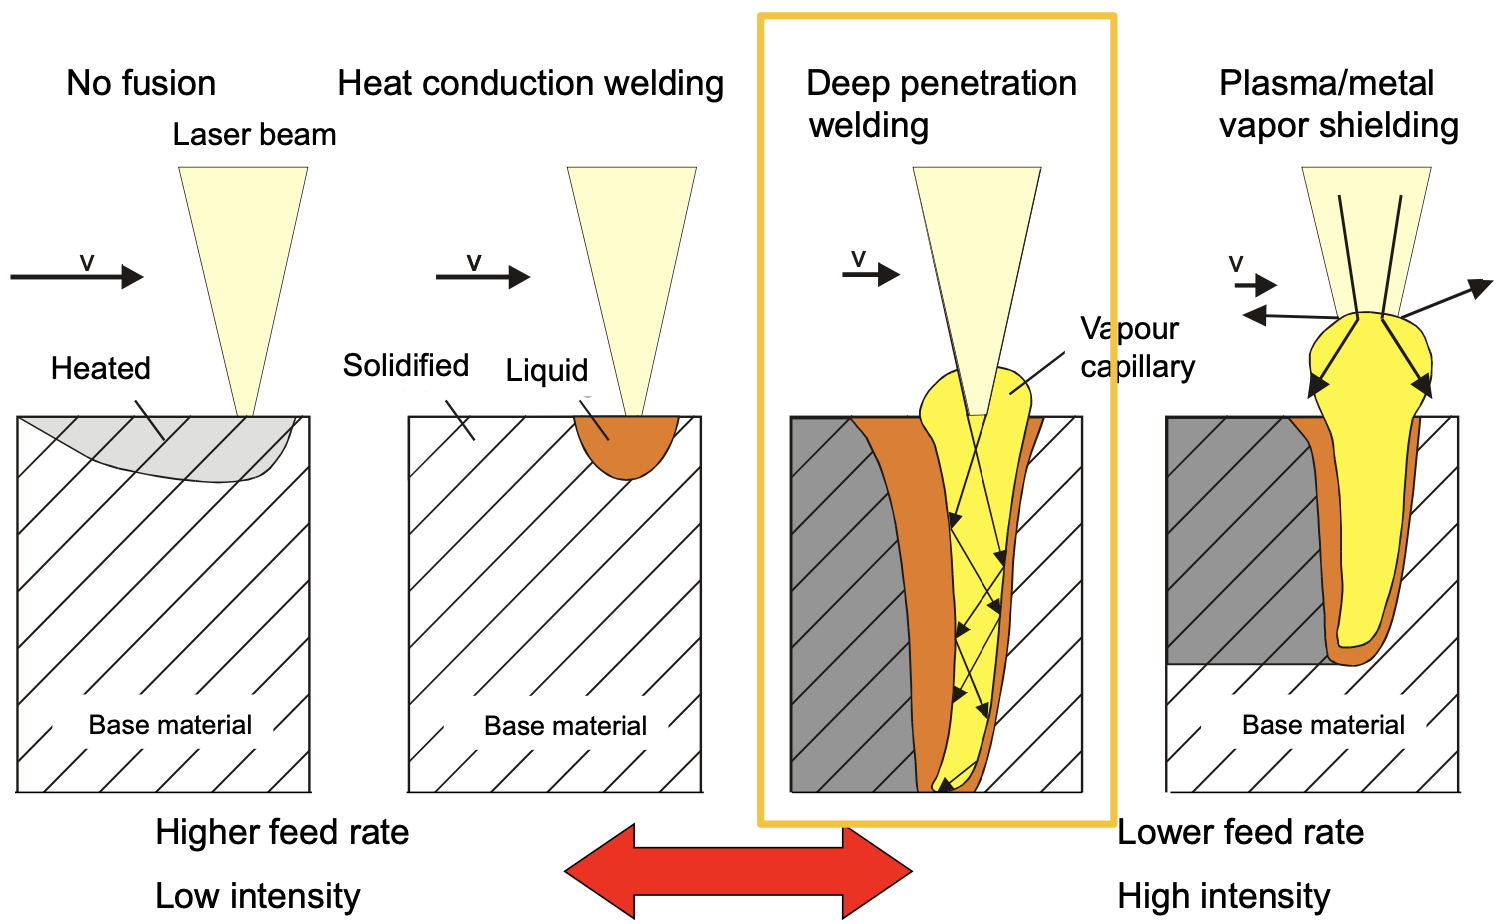
\includegraphics[width=0.45\textwidth]{slike/energy.png}
        \caption{Process of keyhole creation}
        \label{fig:energy}
    \end{subfigure}

    \begin{subfigure}[b]{0.45\textwidth}
        \centering
        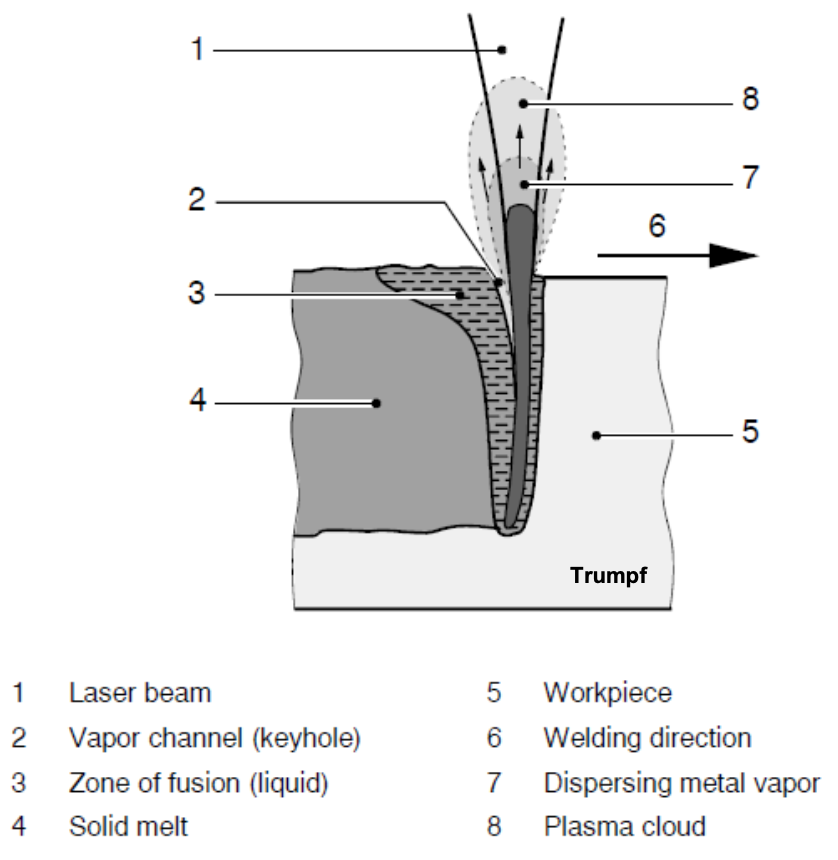
\includegraphics[width=0.45\textwidth]{slike/keyhole_parts.png}
        \caption{Scheme.\sln}
        \label{fig:KHparts}
    \end{subfigure}
\end{figure}

\subsection{Issues in laser welding}

\subsubsection{Humping}
Melt pool fluid dynamics - turbolence - can cause instability on the surface of the weld - \textit{humps}. This process
is called humping, shown on figure \ref{fig:humping}. 
\begin{figure}[h!]
    \centering
    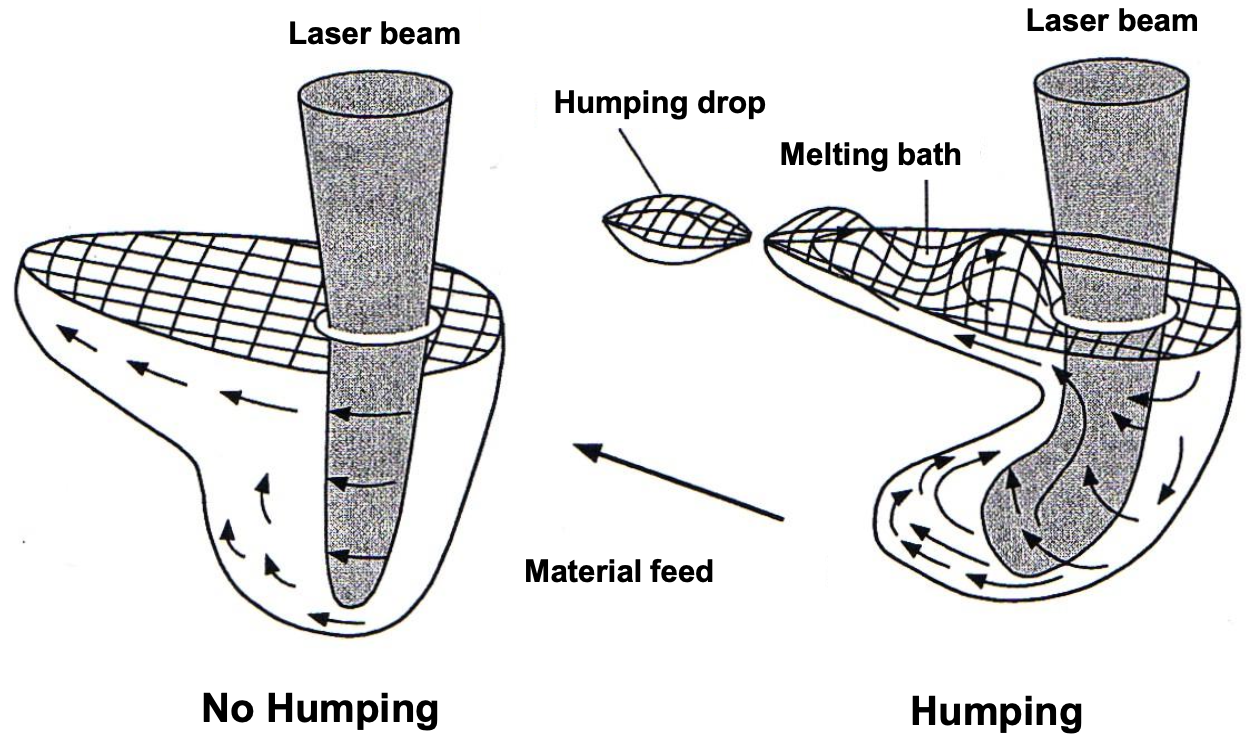
\includegraphics[width=0.5\textwidth]{slike/humping.png}
    \caption{Weld with and -out humping. \sln}
    \label{fig:humping}
\end{figure}

Humping effect limits the speed at which we can weld and badly influences the integrity of the weld.

\subsubsection{Crystallographic changes}
Structure of steel ($Fe, C$) depends on the temperature and concentration.
During welding, structure changes occur. Once during heating and later during cooling down. 
Depending on the speed of the speed of heating/cooling different structures will be present in the metal.
Changes in microstructure have an impact on strength of the weld. They decrease the strength and ductilliy 
of the material. Figure \ref{fig:mustr}
\begin{figure}[h!]
    \centering
    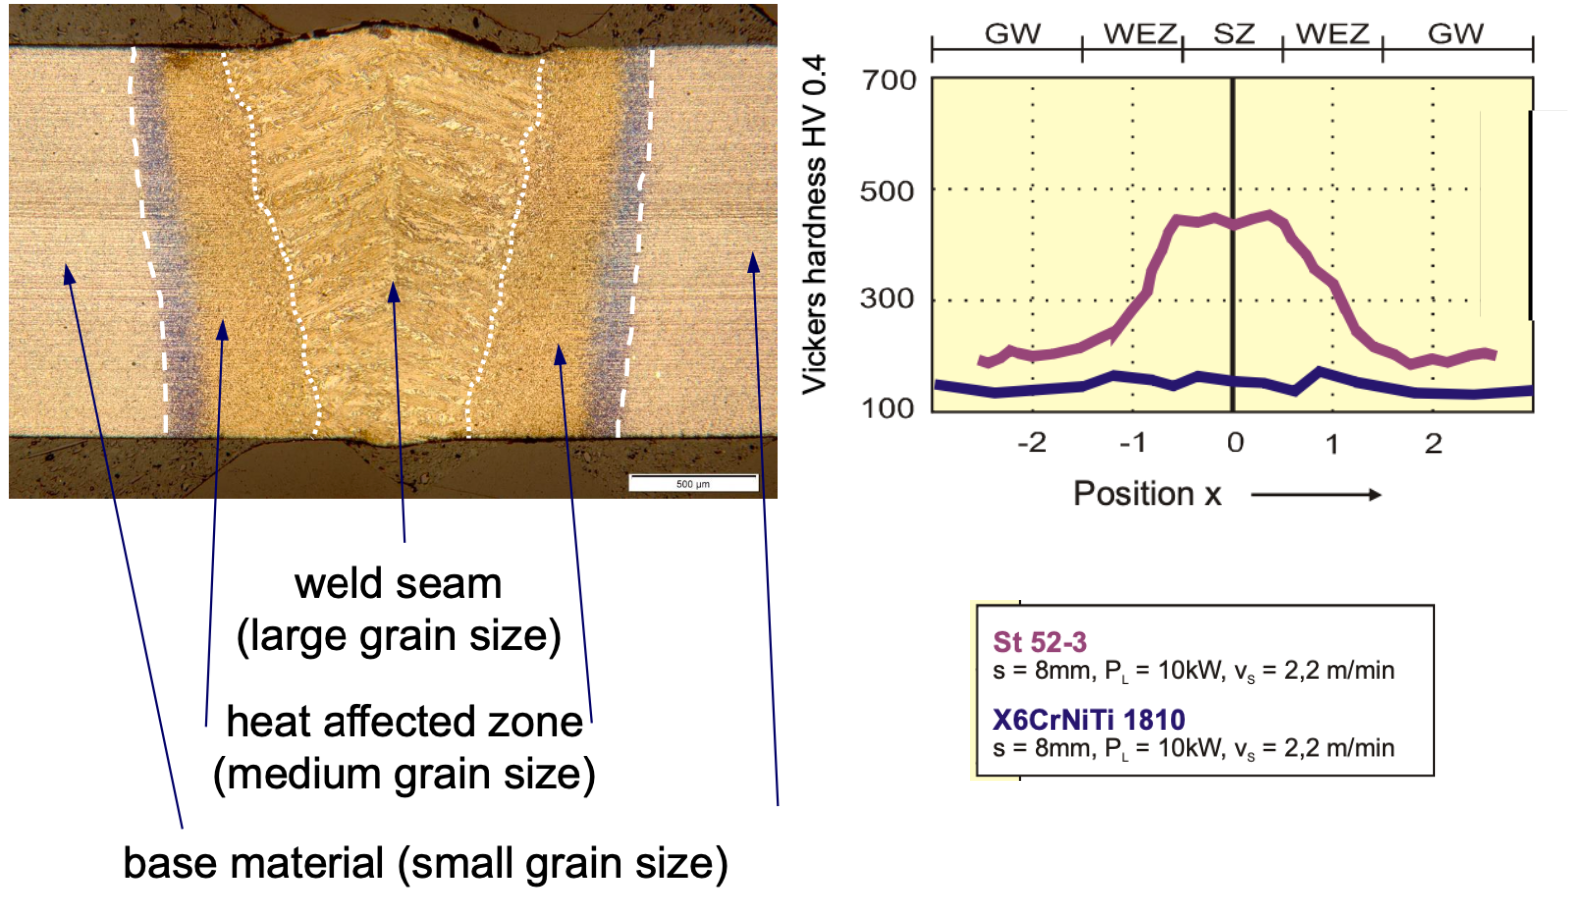
\includegraphics[width=0.75\textwidth]{slike/weld_mstr.png}
    \caption{Weld microstructure. \sln}
    \label{fig:mustr}
\end{figure}
 
\subsubsection{Welding geometry issues}
Welding two metal sheets, which were galvanized in zinc to prevent corrosion,
will cause issues due to the geometric separation of the sheets. Zinc evaporates before the steel melts, so 
we have to leave a gap for the gas to escape.

\subsection{Advantages of laser welding}
Laser welding can reduce or eliminate flanges compared to spot welding. The welding area needs to only be
accessible form on side, meaning we can use smaller enclosed components (e.g. tubes). It also reduces the HAZ and other material distorsions.
in materials. Processing speed is high, and the entire process is controllable and contact free. Depth of penetration can be controlled, we can crate 
welds without them being cosmetically seen from the other side. 
The process is also suitable for automation.


\subsection{Designs suitable for laser welding}
Figures \ref{fig:ge1} show good and bad designs for laser welding.

\begin{figure}[h!]
    \centering
    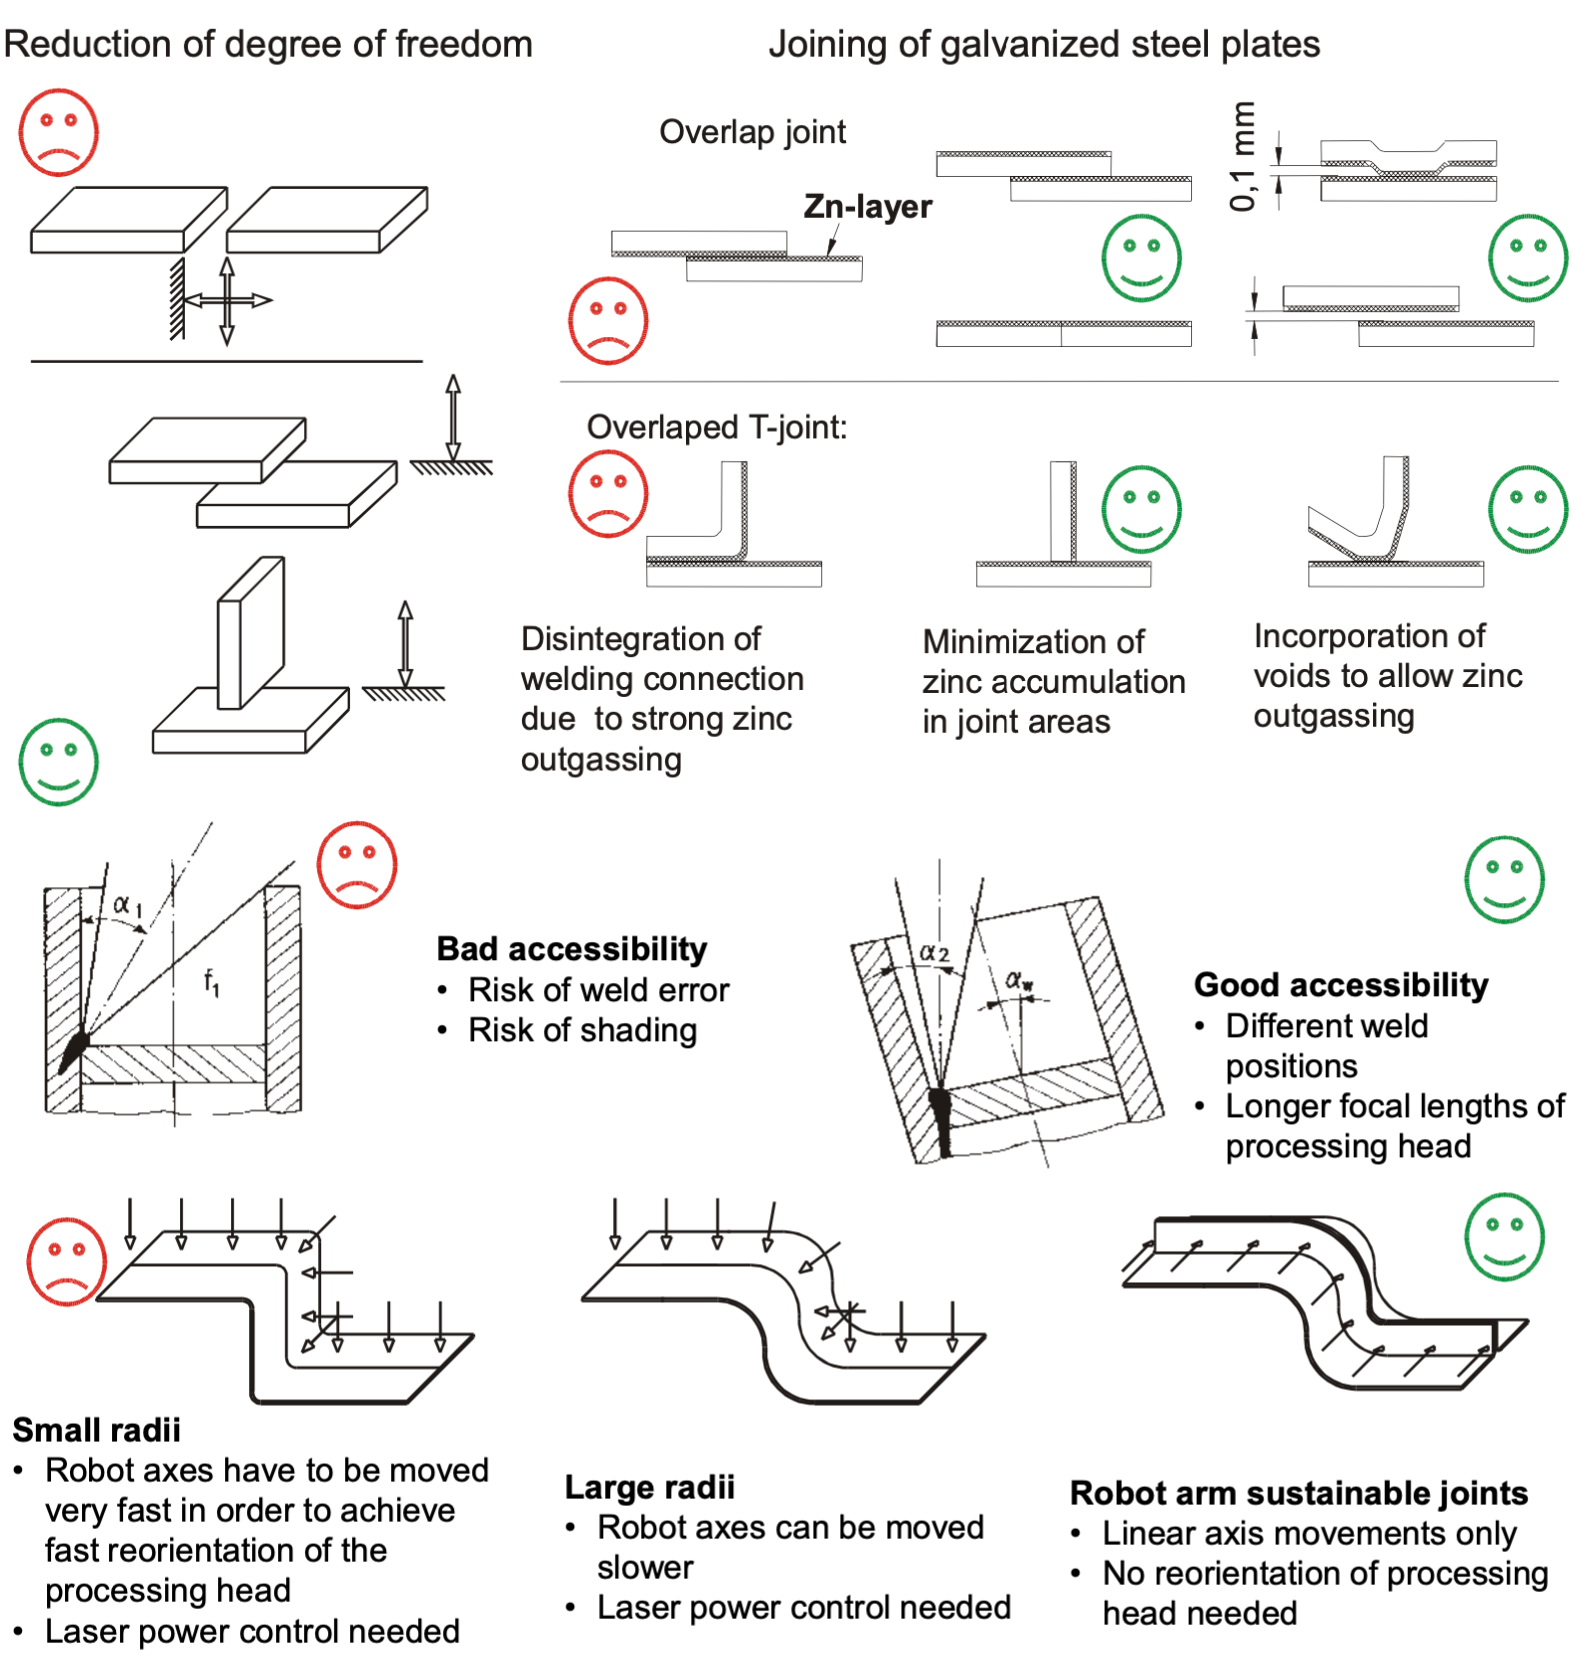
\includegraphics[width=0.75\textwidth]{slike/ge.png}
    \caption{}
    \label{fig:ge1}
\end{figure}

\section{Laser Beam Brazing (Hartlöten)}

Soldering is differentiated based on the temperature of the liquid solder. Table \ref{tab:soldering}
\begin{table}[h!]
    \centering
    \begin{tabular}{|c|c|}
        \hline
        Soft-soldering &$ T \le 450$ \\
        \hline
        Hard-soldering &  $450\le T \le 900$\\
        \hline
        High temp. sold. & $ 900  < T$ \\
        \hline
    \end{tabular}
    \caption{Soldering}
    \label{tab:soldering}
\end{table} 

Process sequence:
\begin{enumerate}
    \item Heating-up of the joining partners, the filler material and the flux
    \item Activation of the flux/protective gas: Removal of surface oxides
    \item Melting of the filler metal
    \item Wetting of the joining partners
    \item Diffusion processes: Forming of mixed crystals or intermediate compounds
\end{enumerate}

Characteristics:
\begin{itemize}
    \item Joint partners only warmed, only filler material is molten
    \item Mechanical strength of joint comparable to that of the filler material
    \item Position and height of the brazing joint are highly influenced by the temperature distribution on the workpieces and the amount of filler material
\end{itemize}

Base material temperature influences the solder surface tension, which can influence the joint strength. 
We \textit{have to} heat up the main parts as well as the solder.

\section{Laser soldering}

Laser soldering is a selective soldering process.
 During the soldering process, the
filler metal or alloy is heated to melting temperatures less than 450 °C. 
Molten soldering paste or solder deposits flows in between the two closely fitted joining
materials. Laser diodes, with power output of less than 100 W are usually used. 
Figure \ref{fig:lsol} show the process.

\begin{figure}[h!]
    \centering
    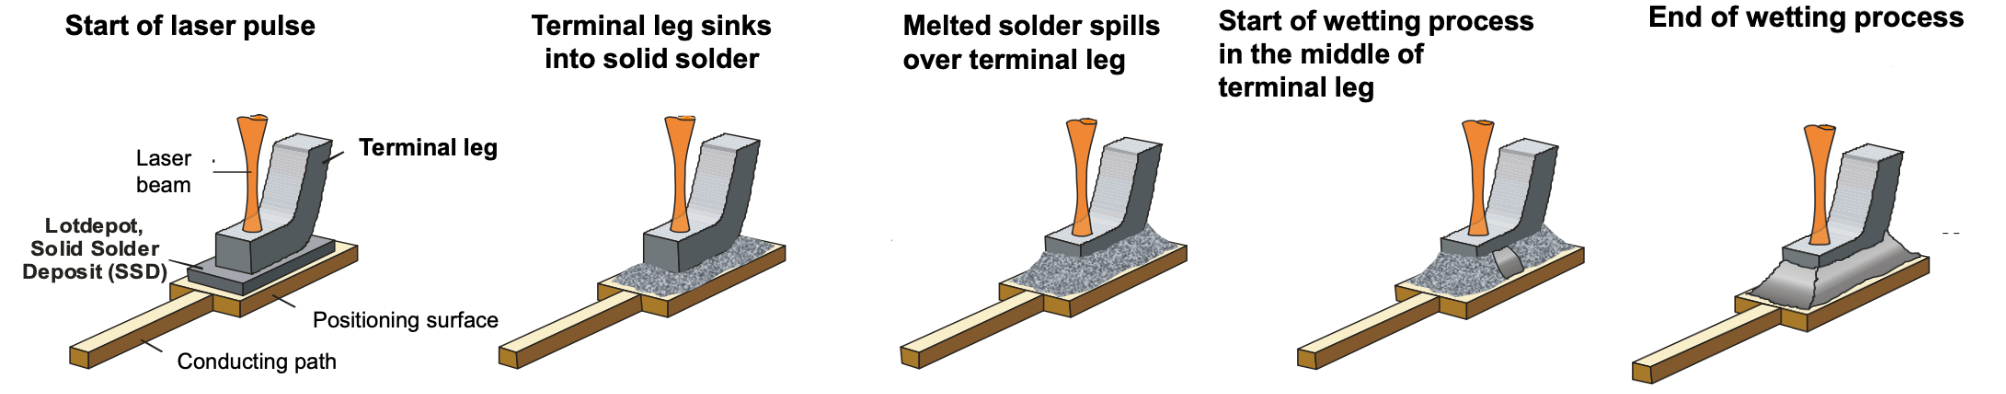
\includegraphics[width=0.95\textwidth]{slike/lassol.png}
    \caption{Laser soldering}
    \label{fig:lsol}
\end{figure}

Compared to welding soldering  has smaller strength of the joint compared to the base material and smaller corrosion resistance 
than the base material. Benefits of soldering are that we can join heat sensitive components, we can reverse the soldering process, and we can join material that do not mix.

\section{Plastics welding}

For laser welding, we can only use \textbf{thermoplastics}. Material has to be meltable, overlapping melting temperature range of joining parts,
and it has to absorb the laser wavelength and convert it to heat.
Mechanism that joins the material is \textit{diffusion}, which is time and heat dependent - this sets the 
highers possible speed. For transparent materials, we have to add additives that absorb NIR light - so we can weld transparent plastics.

\subsection{Process types}
\begin{table}[h!]
    \begin{tabular}{|p{0.31\textwidth} |p{0.31\textwidth}| p{0.31\textwidth}|}
        \hline
        \textbf{Contour welding with focused laser beam} & \textbf{Quasi simultaneous welding with focused laser beam} & \textbf{Simultaneous welding} \\
        \hline
        Suitable for large components & Limited working area & Tailored light so that the complete path is illuminated \\
        Suitable for 2 an 3D & Only 2D contours &  Only 2D contours \\
        Highly localized welding & Melt overflow & Melt overflow \\
        Low cost is the priority & Priority is process control  & Good gap-bridging ability \\
        Can be temperature controlled & Short cycle time & Low flexibility, simple paths \\
        & Large quantities & \\
        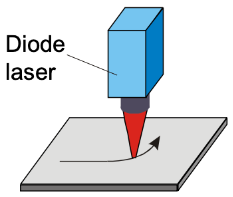
\includegraphics[width=0.3\textwidth]{slike/conturWeld.png} & 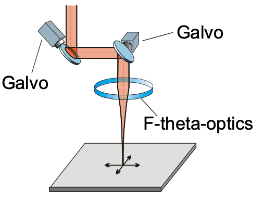
\includegraphics[width=0.3\textwidth]{slike/galvoweld.png} & \\
        \hline
    \end{tabular}
\end{table}

\section*{} % remove the gap !